\documentclass{report}
\usepackage{homework}
\usepackage[table,xcdraw]{xcolor}
\solstrue

\graphicspath{{images/}}

\renewcommand{\hmwkTitle}{Homework 7}

\begin{document}
\mktitle


\begin{problem}

Consider the following network of routers where the numbers above each link indicate link costs:
\begin{center}
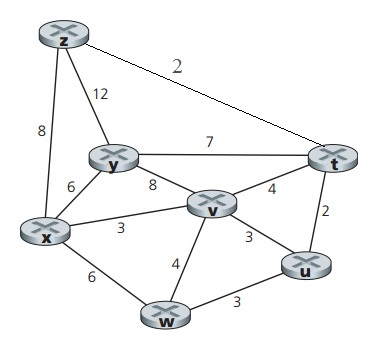
\includegraphics[scale = 0.7]{hw7-topo.jpg}
\end{center}

Considering calculations from the perspective of node \textbf{z}:

\begin{enumerate}
\item Show a table showing iterations of the Link State routing algorithm.
\item Show a resulting routing table (next hop for each destination).
\end{enumerate}

1.
\begin{table}[ht]
\begin{tabular}{cccccccc}
\hline
Node                   & \multicolumn{7}{c}{Iteration}                                                                                                                                                                                                                                                                                  \\ \hline
\multicolumn{1}{c|}{}  & 0                                 & 1                                 & 2                                       & 3                                            & 4                                               & 5                                            & 6                                            \\ \cline{2-8} 
\multicolumn{1}{c|}{t} & $\infty$                          & {\color[HTML]{FD6864} \textbf{2}} & \textbf{2}                              & \textbf{2}                                   & \textbf{2}                                      & \textbf{2}                                   & \textbf{2}                                   \\
\multicolumn{1}{c|}{u} & $\infty$                          & $\infty$                          & {\color[HTML]{FD6864} \textbf{2+2=4}}   & \textbf{4}                                   & \textbf{4}                                      & \textbf{4}                                   & \textbf{4}                                   \\
\multicolumn{1}{c|}{v} & $\infty$                          & $\infty$                          & 2+4=6                                   & {\color[HTML]{FD6864} \textbf{min(6,4+3)=6}} & \textbf{6}                                      & \textbf{6}                                   & \textbf{6}                                   \\
\multicolumn{1}{c|}{w} & $\infty$                          & $\infty$                          & $\infty$                                & 4+3=7                                        & {\color[HTML]{FD6864} \textbf{min(7,6+4)=7}}    & \textbf{7}                                   & \textbf{7}                                   \\
\multicolumn{1}{c|}{x} & $\infty$                          & 8                                 & 8                                       & 8                                            & min(8,6+3)=8                                    & {\color[HTML]{FD6864} \textbf{min(8,7+6)=8}} & \textbf{8}                                   \\
\multicolumn{1}{c|}{y} & $\infty$                          & 12                                & min(12,2+7)=9                           & 9                                            & min(9,6+8)=9                                    & 9                                            & {\color[HTML]{FD6864} \textbf{min(9,8+6)=9}} \\
\multicolumn{1}{c|}{z} & {\color[HTML]{FD6864} \textbf{0}} & \textbf{0}                        & \textbf{0}                              & \textbf{0}                                   & \textbf{0}                                      & \textbf{0}                                   & \textbf{0}                                     
\end{tabular}
\end{table}
\end{problem}

2.
\begin{table}[ht]
\begin{tabular}{cc}
\hline
Destination            & Next Hop \\ \hline
\multicolumn{1}{c|}{t} & t        \\
\multicolumn{1}{c|}{u} & t        \\
\multicolumn{1}{c|}{v} & t        \\
\multicolumn{1}{c|}{w} & t        \\
\multicolumn{1}{c|}{x} & x        \\
\multicolumn{1}{c|}{y} & t        \\
\multicolumn{1}{c|}{z} & z
\end{tabular}
\end{table}

\clearpage
\begin{problem}

Consider a network of 4 routers running Distance Vector routing algorithm where the numbers above each link indicate link costs.
\begin{center}
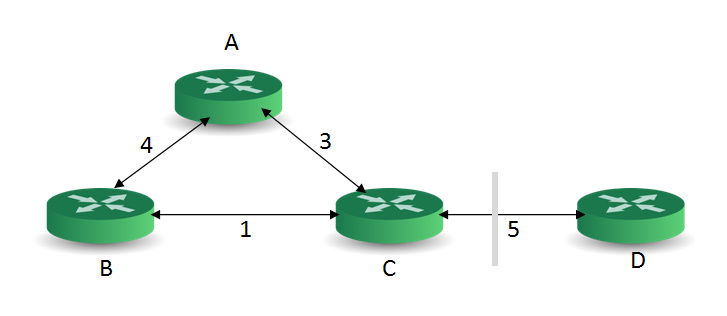
\includegraphics[scale=0.4]{hw7-q2.jpg}
\end{center}

\begin{enumerate}
\item Suppose, the link between C and D fails. Show that split horizon will not eliminate the count-to-infinity problem.
\item How can split horizon with poisoned reverse help in eliminating the count-to-infinity problem when the link between C and D fails?
\end{enumerate}

\begin{answer}{30em}
  \begin{enumerate}
    \item With split horizon, A would not advertise to C its route to D (through
      C). Likewise, B would not advertise to C its route to D (through C).
      However, A and B will advertise their routes to D to each other, such that
      when the link from C to D fails, they will try to use each other's routes
      to reach D, and begin counting to infinity.

    \item Split horizion with poison reverse works by making each node advertise
      a route as unreachable over the same interface through which it learns
      that route, in addition to the traditional split horizion approach. In
      this example, when A learns of its route to D, it will broadcast to B and
      C that it cannot reach D. Likewise, when B learns of its route to D,
      it will tell A and C that it cannot reach D. Thus, when the link between
      C and D breaks, A and B will not try to reach D by going through each
      other.
  \end{enumerate}

\end{answer}


\end{problem}

\clearpage
\begin{problem}
Consider a network of 6 routers shown in the figure below. The network is running OSPF routing protocol and the cost of each is 10. Each router is announcing a single unique prefix (prefix A, prefix B, ... prefix F). Propagation delay for each link is 10 msec. When a router has to choose between two or more equal cost paths to
the same destination, it breaks the tie by picking them in an alphabetic order). The network has been up and running for a long time. However, at time T=100 min, we observe that
link A-F fails.

\begin{center}
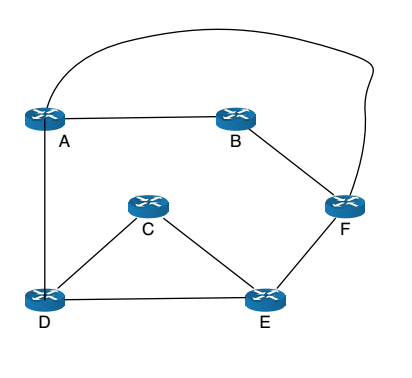
\includegraphics[scale=0.5]{hw7-ospf.png}
\end{center}
\begin{enumerate}
\item How will node A and node F discover that the link A-F has failed? \\ \\

\begin{answer}{5em}
Node A and Node F will discover that the link A-F has failed when their
heartbeat requests time out.
\end{answer}

\item How will node C discover that the link A–F has failed? Will this affect C's routing table? \\ \\

\begin{answer}{5em}
  Node C discovers that link A-F has failed as the information of its failure
  propagates through the network. It will not affect C's routing table because
  C can still reach A and F in 20 ms, just as before. The A-F link wasn't really
  being used by Node C.
\end{answer}

\item Overall, how many updates will be generated and propagated in the network as a result of this failure (i.e., not considering periodic updates)? Describe why. \\ \\
\begin{answer}{6em}
  8 updates will be generated as the network uses a simple flooding to algorithm
  to propagate link state messages. A will generate 2 updates to inform its neighbors B and
  D, F will genererate 2 updates to inform its neighbors B and E. Then D will
  generate 2 more updates to inform its neighbors C ane E, and E will generate
  2 more updates to inform its neighbors C and D. This is a total of 8 updates.
\end{answer}
\item Which routers will make a change in their routing table as a result of this failure? \\ \\
\begin{answer}{6em}
  Routers A and F, will have to change their routing tables for obvious reasons,
  after the link went down it will take 20ms for them to relay messages instead
  of 10. Router D will have to update its tables, as the route D-F used the A-F
  link (D-A-F, tie broken by alphabetic order). For the same reason, Router E will not have to update
  its tables because it was not using the A-F link (it uses E-D-A).
\end{answer}
\end{enumerate}

\end{problem}


\clearpage
\begin{problem}
Consider the network shown below. Suppose AS3 and AS2 are running OSPF
for their intra-AS routing protocol. Suppose AS1 and AS4 are also running OSPF
for their intra-AS routing protocol. Suppose eBGP and iBGP are used for the
inter-AS routing protocol. Initially suppose there is no physical link between
AS2 and AS4.

\begin{center}
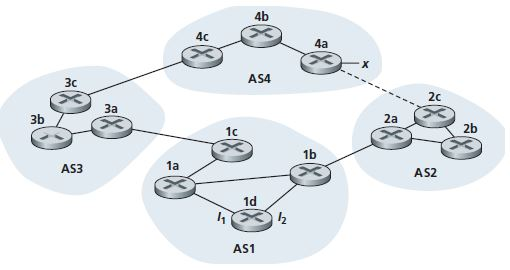
\includegraphics{hw7-q4}
\end{center}

At some time T, the prefix $x$ appears in AS4, adjacent to the router 4a.
From which routing protocol (OSPF, eBGP, or iBGP):

\begin{enumerate}
\item Router 3c learns about prefix $x$? 
\item Router 3b learns about prefix $x$?
\item Router 4a learns about prefix $x$?
\item Router 1d learns about prefix $x$?
\end{enumerate}

\begin{answer}{10em}

\begin{enumerate}
  \item eBGP
  \item iBGP
  \item iBGP
  \item OSPF
\end{enumerate}

\end{answer}


\end{problem}



\end{document}
